\documentclass{article}
\usepackage{graphicx} % Required for inserting images
\graphicspath{ {./Images/} }
\usepackage{pdfpages}
\newcommand{\insertslide}[2]{
\begin{center}
    \fbox{\includegraphics[page=#2,scale=0.25]{#1}}
\end{center}
}
% \insertslide{Slides/CM1.pdf}{1} to insert first page of CM1.pdf, for example.
\usepackage{amsmath}
\renewcommand{\familydefault}{\sfdefault}

\title{Notes LMAPR1230}
\author{Quentin Bodart}
\date{Q1 2024-2025}

\begin{document}
\maketitle
\tableofcontents
\pagebreak

\section*{Compétences visées}
    \begin{itemize}
        \item Utiliser correctement le langage de la chimie et plus
        particulièrement celui de la chimie organique.
        \item Comprendre les relations entre la nature, la
        structure et les propriétés de composés organiques.
        \item Prédire et analyser la réactivité de composés
        organiques donnés.
        \item Pouvoir utiliser les notions théoriques apprises au
        cours pour résoudre des exercices.
    \end{itemize}

\section{CM 1 : Introduction et rappels}
    \subsection{La chimie organique}
        La chimie organique est une branche de la chimie qui concerne
        l’étude et la transformation de molécules d’origine pétrolière ou
        vivante contenant principalement
        du carbone, de l’hydrogène, de l’oxygène et de l’azote.\\\\
        Elle prend ses débuts dans la création accidentelle d'urée par Friedrich Wöhler en 1828.
        Cette découverte mit fin à la théorie "vitaliste" (seule la nature est capable de synthétiser des molécules organiques) 
        et marque le début de la synthèse artificielle de ces molécules.

    \subsection{Le carbone}
        \subsubsection{Pourquoi le carbone?}
            Pourquoi le carbone est-il prépondérant dans la chimie organique ? \\
            D'autant plus que carbone est très peu abondant à l'échelle de l'univers (0,06 \%) !

            \begin{itemize}
                \item La liaison C-C est particulièrement forte (+- 350 kJ/mol, contre 230 pour Si-Si, 146 pour O-O, ...)
                \item Les liaison C=C sont moins fortes que C-C, ce qui fait que le carbone tend 
                    à former de longues chaînes (contrairement aux autres atomes)
                \item Il se lie très fort avec H
            \end{itemize}
            Donc, l'état "préféré" du carbone est une longue chaîne, parfois branchée 
            et se repliant sur elle-même, et fortement liée avec des atomes d'hydrogène.
        
        \subsubsection{Hybridation}
            Les liaison du carbone ne peuvent pas simplement 
            s'expliquer via ses électrons de valence !
            Le carbone s'hybride, formant des orbitales $sp$, $sp^2$ ou $sp^3$ ! \\
            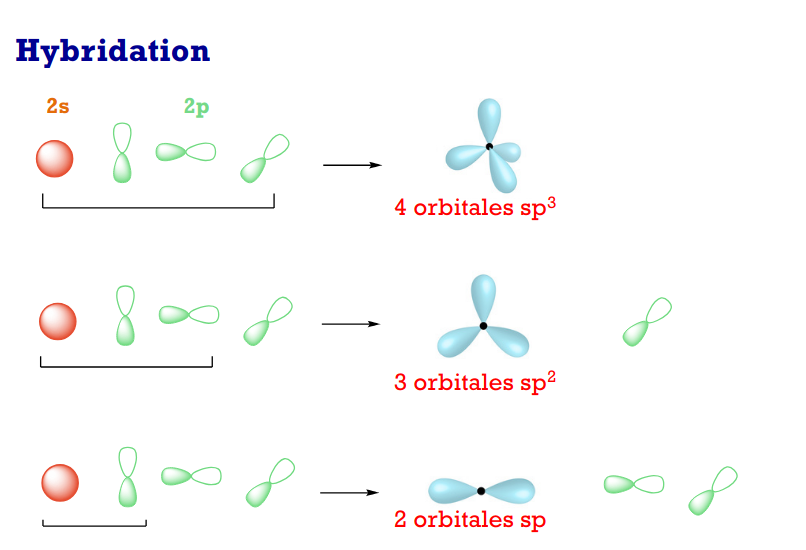
\includegraphics[scale=.5]{hybridation_carbone.png} \\
            Les orbitales $p$ restantes vont former des liaisons 
            nommées $\pi$ entre elles, tandis que les orbitales $sp$ 
            vont se lier en formant de liaisons $\sigma$. \\\\
            La liaison C=C généralement formée d'une liaison $\pi$ 
            et d'une liaison $\sigma$ :\\
            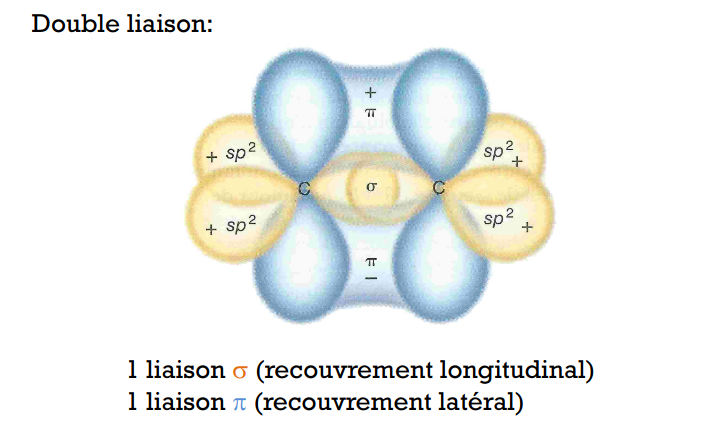
\includegraphics[scale=.5]{liaison_double_c_c.png}\\\\
            La liaison C$\equiv$C, quant à elle, est généralement 
            formée de deux liaison $\pi$ et d'une liaison $\sigma$ : \\
            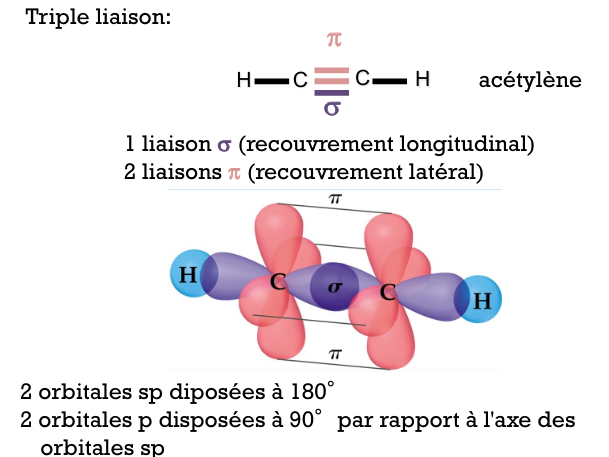
\includegraphics[scale=.5]{liaison_triple_c_c.png}

        

    \subsection{Théorie VSEPR}
        La \textbf{théorie VSEPR} (\textbf{V}alence \textbf{S}hell \textbf{E}lectron \textbf{P}air \textbf{R}epulsion)
        vise à prédire la géométrie d'une molécule en se basant sur les
        répulsions entre paires d'électrons. \\\\
        On y considère qu'un atome est entouré d'électrons de valences répartis 
        par \textbf{paires}, et que la molécule tente d'adopter une 
        géométrie \textbf{minimisant la répulsion entre ces paires} :\\
        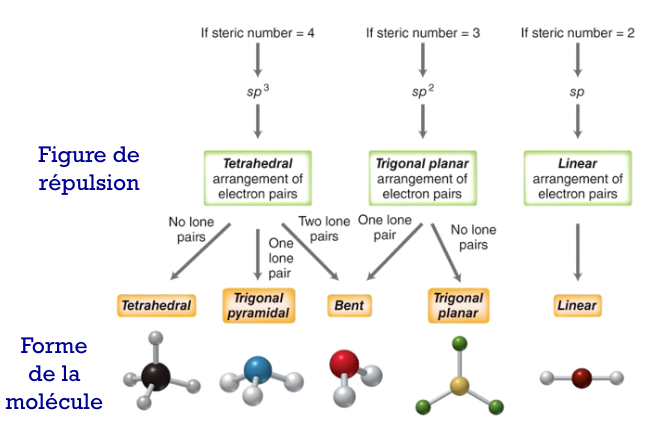
\includegraphics[scale=.7]{VSEPR.png}

    \subsection{Représenter une molécule}
        \subsubsection{Formules}
            Il y a plusieurs manières de représenter une molécule :
            \begin{itemize}
                \item Formule Brute : Liste simplement les atomes présents \\
                Exemple : $C_2 H_6 O$, $C_3 H_6 Cl_2$, ... 
                \item Formule Semi-dévellopée : Liste les atomes dans l'ordre de la chaîne principale \\
                Exemple : $CH_3CH_2OH$, $CH_2ClCHClCH_3$, $CH_3CH_2CH_2CH_2CH_3$, ... 
                \item Formule dévellopée plane (structure de Lewis) : Représente les molécules à plat et les liaisons entre groupements (Expliquée plus bas)\\
                Exemple :\\
                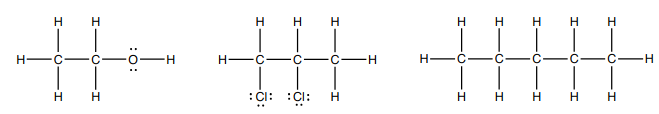
\includegraphics[scale=.6]{structures_planes.png}
                \item Formule simplifiée (ou topologique) : chaque coin représente un carbone lié à un maximum d'atomes d'hydrogène \\
                Exemple :\\
                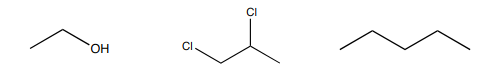
\includegraphics[scale=.8]{formule_topologique.png}
            \end{itemize}
        
        \subsubsection{Structure de Lewis}
            Elle se base sur la règle de l'octet, et permet de représenter les \textbf{charges formelles} : \\
            % TODO
            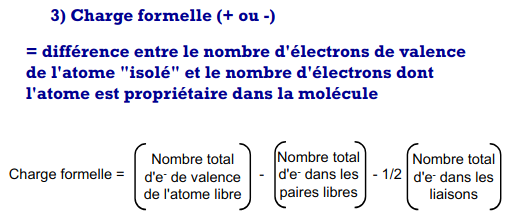
\includegraphics{charge_formelle.png}

    \subsection{Les hydrocarbures}
        \subsubsection{Les alcanes}
            Les alcanes sont des chaînes de C simplement liés et saturés en atomes d'hydrogène. \\
            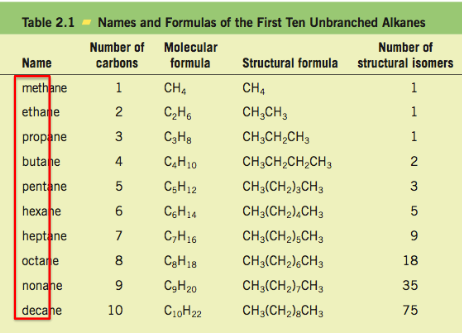
\includegraphics{nomenclature_alcanes.png}
        
        \subsubsection{Nomenclature}
            La nomenclature des alcanes passe par les
            règles \textbf{IUPAC} (International Union for Pure and Applied Chemistry) :\\
            \begin{itemize}
                \item Le préfixe est lié à la longueur de chaîne.
                \item Le suffixe “ane” signifie hydrocarbure saturé.
                \item On sélectionne la chaîne la plus longue.
                \item On numérote cette chaîne de façon à avoir les plus petits chiffres
                possibles pour spécifier la position des substituants
                \item Les substituants sont affectés du numéro(s) du (des) carbone(s)
                porteur(s) pour les localiser
                \item Les préfixes di-, tri-, tétra-,… sont utilisés si un même substituant
                est présent plusieurs fois
            \end{itemize}

        \subsubsection{Groupes alkyles}
            Les ramifications à base de C et H retrouvés autour de la chaîne principale sont des \textbf{groupes alkyles} :\\
            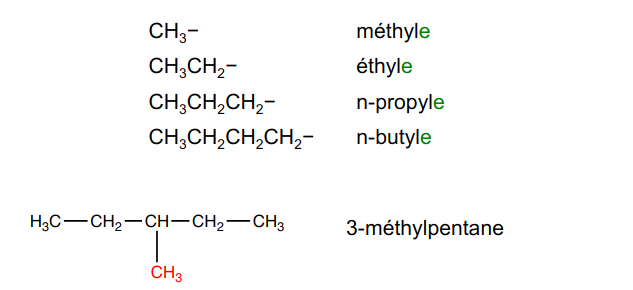
\includegraphics[scale=.4]{groupes_alkyles.png}
            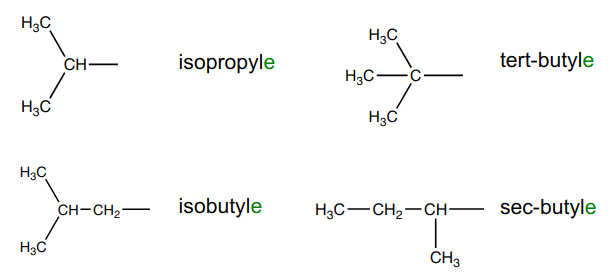
\includegraphics[scale=.4]{groupes_alkyles_particuliers.png}

        \subsubsection{Alcanes Cycliques}
            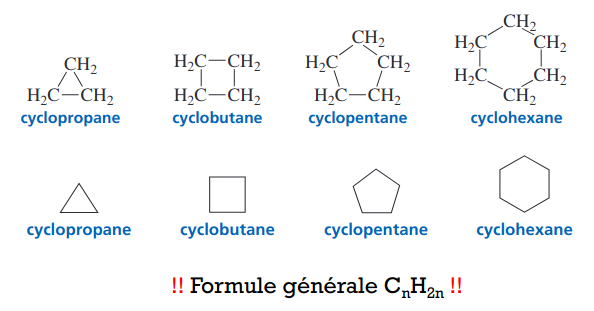
\includegraphics{alcanes_cycliques.png}
        
        %TODO
    \pagebreak
    \subsection{Les groupes fonctionnels}
        \begin{itemize}
            \item Alcools : $R-OH$, Si R = C $sp^2$, on parle d'\textbf{énol}.
            \item Ethers : $R-O-R'$
            \item Amines : $N-R_3$
            \item Cétones : \\ 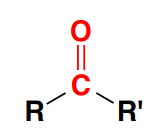
\includegraphics[scale=.5]{cetone.png}
            \item Aldéhydes : \\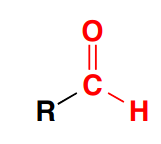
\includegraphics[scale=.5]{aldehyde.png}
            \item Acides carboxyliques : \\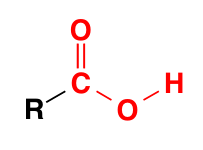
\includegraphics[scale=.5]{acide_carboxylique.png}
            \item Esters : \\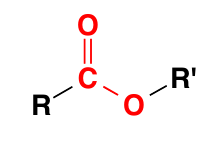
\includegraphics[scale=.5]{ester.png}
            \item Amides : \\
            %TODO
        \end{itemize}

\section{CM 2 : Isomérie}
    \subsection{Isomères de constitution}
        Les isomères de constitution sont des composés qui ont
        la même formule brute (moléculaire) mais une structure
        différente.\\
        Il en existe trois types:
        \begin{itemize}
            \item Isomères de chaîne
            \item Isomères de position
            \item Isomères de fonction
        \end{itemize}
        Exemple d'isomère de chaîne:
        \insertslide{Slides/CM2.pdf}{3}
        Exemple d'isomère de position:
        \insertslide{Slides/CM2.pdf}{4}
        Exemple d'isomère de constitution:
        \insertslide{Slides/CM2.pdf}{5}

    \subsection{Stéréoisomérie}
        La stéréochimie est le domaine de la
        chimie qui étudie les représentations 3D
        des molécules ainsi que les mécanismes
        de réaction en 3D.\\\\
        Des molécules qui ont une connectivité
        entre atomes identique mais un
        arrangement spatial différent sont
        appelées des stéréoisomères.\\\\
        Exemple de stéréoisomère :
        \insertslide{Slides/CM2.pdf}{7}
        
        \subsubsection{Chiralité}
            Une molécule est \textbf{chirale} si elle n'est pas
            superposable à son image miroir.
            Dans le cas de la slide précédente, ce sont des molécules \textbf{chirales}
            car elles ne peuvent pas se superposer (à droite)\\\\
            Un autre exemple de molécule / groupement chiral sont les acides aminés:\\
            \insertslide{Slides/CM2.pdf}{10}

    \subsection{Centre stéréogénique}
        Une molécule chirale contient un ou plusieurs
        centre(s) asymétrique(s).\\
        Un atome de carbone hybridé sp 3 portant
        quatre atomes ou groupes d'atomes différents
        est un atome de carbone asymétrique.\\
        On parle alors de \textbf{centre stéréogénique} :
        \insertslide{Slides/CM2.pdf}{16}
        Si la molécule contient un plan ou centre de symétrie ou contient au moins deux fois le
        même groupement/atome, il est fort probable qu'elle soit achirale, et que le centre
        \textbf{ne soit pas stéréogénique} :
        \insertslide{Slides/CM2.pdf}{13}

    \subsection{Enantiomères}
    Une molécule chirale et son image miroir sont
    appelées des \textbf{énantiomères}.
    Un mélange 50/50 de deux énantiomères est
    appelé \textbf{mélange racémique}.\\
    Lorsque l'on est en présence d'un seul des énantiomères, on
    dira que le composé est \textbf{optiquement pur}.

        \subsubsection{Convention R-S}
            \textbf{Régles de Cahn, Ingold et Prelog} :
            \begin{itemize}
                \item Les quatre atomes directement liés au carbone
                asymétrique sont classés par ordre de Z décroissant.
                \item Si au moins deux des quatre atomes sont identiques,
                il faut progresser de voisin en voisin afin de déterminer
                la priorité.\\
                Dans ce cas, il ne faut \textbf{pas additionner les Z} !\\
                Par exemple, C lié à OHH aura une plus grand priorité que CCC,
                car O est plus électronégatif :
                \insertslide{Slides/CM2.pdf}{22}
            \end{itemize}
            Après avoir déterminé l'ordre de priorité, il faut représenter
            la molécule de manière à ce qu'elle soit orientée de la manière
            suivante :
            \insertslide{Slides/CM2.pdf}{24}
            Enfin, on attribuera la lettre "R" (du latin, Rectus) ou "S" (du latin, Sinister)
            de la manière suivante:
            \insertslide{Slides/CM2.pdf}{25}
            Une méthode utile serait de permuter les groupements 3 par 3 
            afin de préserver la stéréochimie (représente une rotation de 120°
            autour d'un axe).
            Les permuter, cependant, inverserait la stéréochimie (R$\rightarrow$S ou S$\rightarrow$R).
        
        \subsubsection{Plus d'un centre asymétrique?}
            Lorsqu'une molécule contient plus d'un centre asymétrique, les 
            stéréoisomères sont séparés en deux catégories :
            \begin{itemize}
                \item Les énantiomères, images miroir, inséparables chimiquement\\
                RR-SS, RS-SR 
                \item Les diastéréoisomères, séparables chimiquement\\
                RR-RS, RR-SR, SS-RS, SS-SR
            \end{itemize}
            Exemple :
            \insertslide{Slides/CM2.pdf}{27}
            \insertslide{Slides/CM2.pdf}{28}
        
        \subsubsection{Projection de Fischer}
            %TODO Expliquer
            \insertslide{Slides/CM2.pdf}{35}

    \subsection{Proriétés des énantiomères}
        En milieu achiral, deux énantiomères ont des propriétés
        identiques (températures de fustion et d'ébulition,
        densité, solubilité…)\\
        Ils présentent cependant des propriétés optiques
        différentes (déviation du plan d’un rayonnement
        éléctromagnétique polarisé).\\
        Deux énantiomères possèdent des pouvoirs rotatoires
        spécifiques opposés.\\
        Un mélange racémique, c’est-à-dire un mélange
        équimolaire d’énantiomères, est donc optiquement
        inactif par compensation.
        On peut mesurer le pouvoir rotatoire spécifique d'un mélange,
        on utilisera la formule suivante:
        \insertslide{Slides/CM2.pdf}{38}
        Si la rotation se fait dans le sens horlogique, on parle de \textbf{dextrogyre} (d,+).\\
        A l'inverse, on parle de \textbf{levogyre} (l,-).\\
        Il n'existe aucun lien entre R,S et le sens de rotation.\\\\
        Autre exemple de différence de propriétés entre les deux énantiomères:
        \insertslide{Slides/CM2.pdf}{41}
        tératogène $\rightarrow$ génère des malformations

        \subsubsection{Notation D-L}
            \insertslide{Slides/CM2.pdf}{43}
            Autres exemples:
            \insertslide{Slides/CM2.pdf}{44}
            \insertslide{Slides/CM2.pdf}{45}

    \subsection{Isomérie géométrique}
        \insertslide{Slides/CM2.pdf}{46}
        \insertslide{Slides/CM2.pdf}{47}
        \insertslide{Slides/CM2.pdf}{48}
    
    \subsection{En résumé}
        \insertslide{Slides/CM2.pdf}{50}
        \insertslide{Slides/CM2.pdf}{51}
    \subsection{Isomérie conformationnelle}
    \subsection{Les cycloalcanes}
\end{document}